\documentclass[1p]{elsarticle_modified}
%\bibliographystyle{elsarticle-num}

%\usepackage[colorlinks]{hyperref}
%\usepackage{abbrmath_seonhwa} %\Abb, \Ascr, \Acal ,\Abf, \Afrak
\usepackage{amsfonts}
\usepackage{amssymb}
\usepackage{amsmath}
\usepackage{amsthm}
\usepackage{scalefnt}
\usepackage{amsbsy}
\usepackage{kotex}
\usepackage{caption}
\usepackage{subfig}
\usepackage{color}
\usepackage{graphicx}
\usepackage{xcolor} %% white, black, red, green, blue, cyan, magenta, yellow
\usepackage{float}
\usepackage{setspace}
\usepackage{hyperref}

\usepackage{tikz}
\usetikzlibrary{arrows}

\usepackage{multirow}
\usepackage{array} % fixed length table
\usepackage{hhline}

%%%%%%%%%%%%%%%%%%%%%
\makeatletter
\renewcommand*\env@matrix[1][\arraystretch]{%
	\edef\arraystretch{#1}%
	\hskip -\arraycolsep
	\let\@ifnextchar\new@ifnextchar
	\array{*\c@MaxMatrixCols c}}
\makeatother %https://tex.stackexchange.com/questions/14071/how-can-i-increase-the-line-spacing-in-a-matrix
%%%%%%%%%%%%%%%

\usepackage[normalem]{ulem}

\newcommand{\msout}[1]{\ifmmode\text{\sout{\ensuremath{#1}}}\else\sout{#1}\fi}
%SOURCE: \msout is \stkout macro in https://tex.stackexchange.com/questions/20609/strikeout-in-math-mode

\newcommand{\cancel}[1]{
	\ifmmode
	{\color{red}\msout{#1}}
	\else
	{\color{red}\sout{#1}}
	\fi
}

\newcommand{\add}[1]{
	{\color{blue}\uwave{#1}}
}

\newcommand{\replace}[2]{
	\ifmmode
	{\color{red}\msout{#1}}{\color{blue}\uwave{#2}}
	\else
	{\color{red}\sout{#1}}{\color{blue}\uwave{#2}}
	\fi
}

\newcommand{\Sol}{\mathcal{S}} %segment
\newcommand{\D}{D} %diagram
\newcommand{\A}{\mathcal{A}} %arc


%%%%%%%%%%%%%%%%%%%%%%%%%%%%%5 test

\def\sl{\operatorname{\textup{SL}}(2,\Cbb)}
\def\psl{\operatorname{\textup{PSL}}(2,\Cbb)}
\def\quan{\mkern 1mu \triangleright \mkern 1mu}

\theoremstyle{definition}
\newtheorem{thm}{Theorem}[section]
\newtheorem{prop}[thm]{Proposition}
\newtheorem{lem}[thm]{Lemma}
\newtheorem{ques}[thm]{Question}
\newtheorem{cor}[thm]{Corollary}
\newtheorem{defn}[thm]{Definition}
\newtheorem{exam}[thm]{Example}
\newtheorem{rmk}[thm]{Remark}
\newtheorem{alg}[thm]{Algorithm}

\newcommand{\I}{\sqrt{-1}}
\begin{document}

%\begin{frontmatter}
%
%\title{Boundary parabolic representations of knots up to 8 crossings}
%
%%% Group authors per affiliation:
%\author{Yunhi Cho} 
%\address{Department of Mathematics, University of Seoul, Seoul, Korea}
%\ead{yhcho@uos.ac.kr}
%
%
%\author{Seonhwa Kim} %\fnref{s_kim}}
%\address{Center for Geometry and Physics, Institute for Basic Science, Pohang, 37673, Korea}
%\ead{ryeona17@ibs.re.kr}
%
%\author{Hyuk Kim}
%\address{Department of Mathematical Sciences, Seoul National University, Seoul 08826, Korea}
%\ead{hyukkim@snu.ac.kr}
%
%\author{Seokbeom Yoon}
%\address{Department of Mathematical Sciences, Seoul National University, Seoul, 08826,  Korea}
%\ead{sbyoon15@snu.ac.kr}
%
%\begin{abstract}
%We find all boundary parabolic representation of knots up to 8 crossings.
%
%\end{abstract}
%\begin{keyword}
%    \MSC[2010] 57M25 
%\end{keyword}
%
%\end{frontmatter}

%\linenumbers
%\tableofcontents
%
\newcommand\colored[1]{\textcolor{white}{\rule[-0.35ex]{0.8em}{1.4ex}}\kern-0.8em\color{red} #1}%
%\newcommand\colored[1]{\textcolor{white}{ #1}\kern-2.17ex	\textcolor{white}{ #1}\kern-1.81ex	\textcolor{white}{ #1}\kern-2.15ex\color{red}#1	}

{\Large $\underline{12n_{0035}~(K12n_{0035})}$}

\setlength{\tabcolsep}{10pt}
\renewcommand{\arraystretch}{1.6}
\vspace{1cm}\begin{tabular}{m{100pt}>{\centering\arraybackslash}m{274pt}}
\multirow{5}{120pt}{
	\centering
	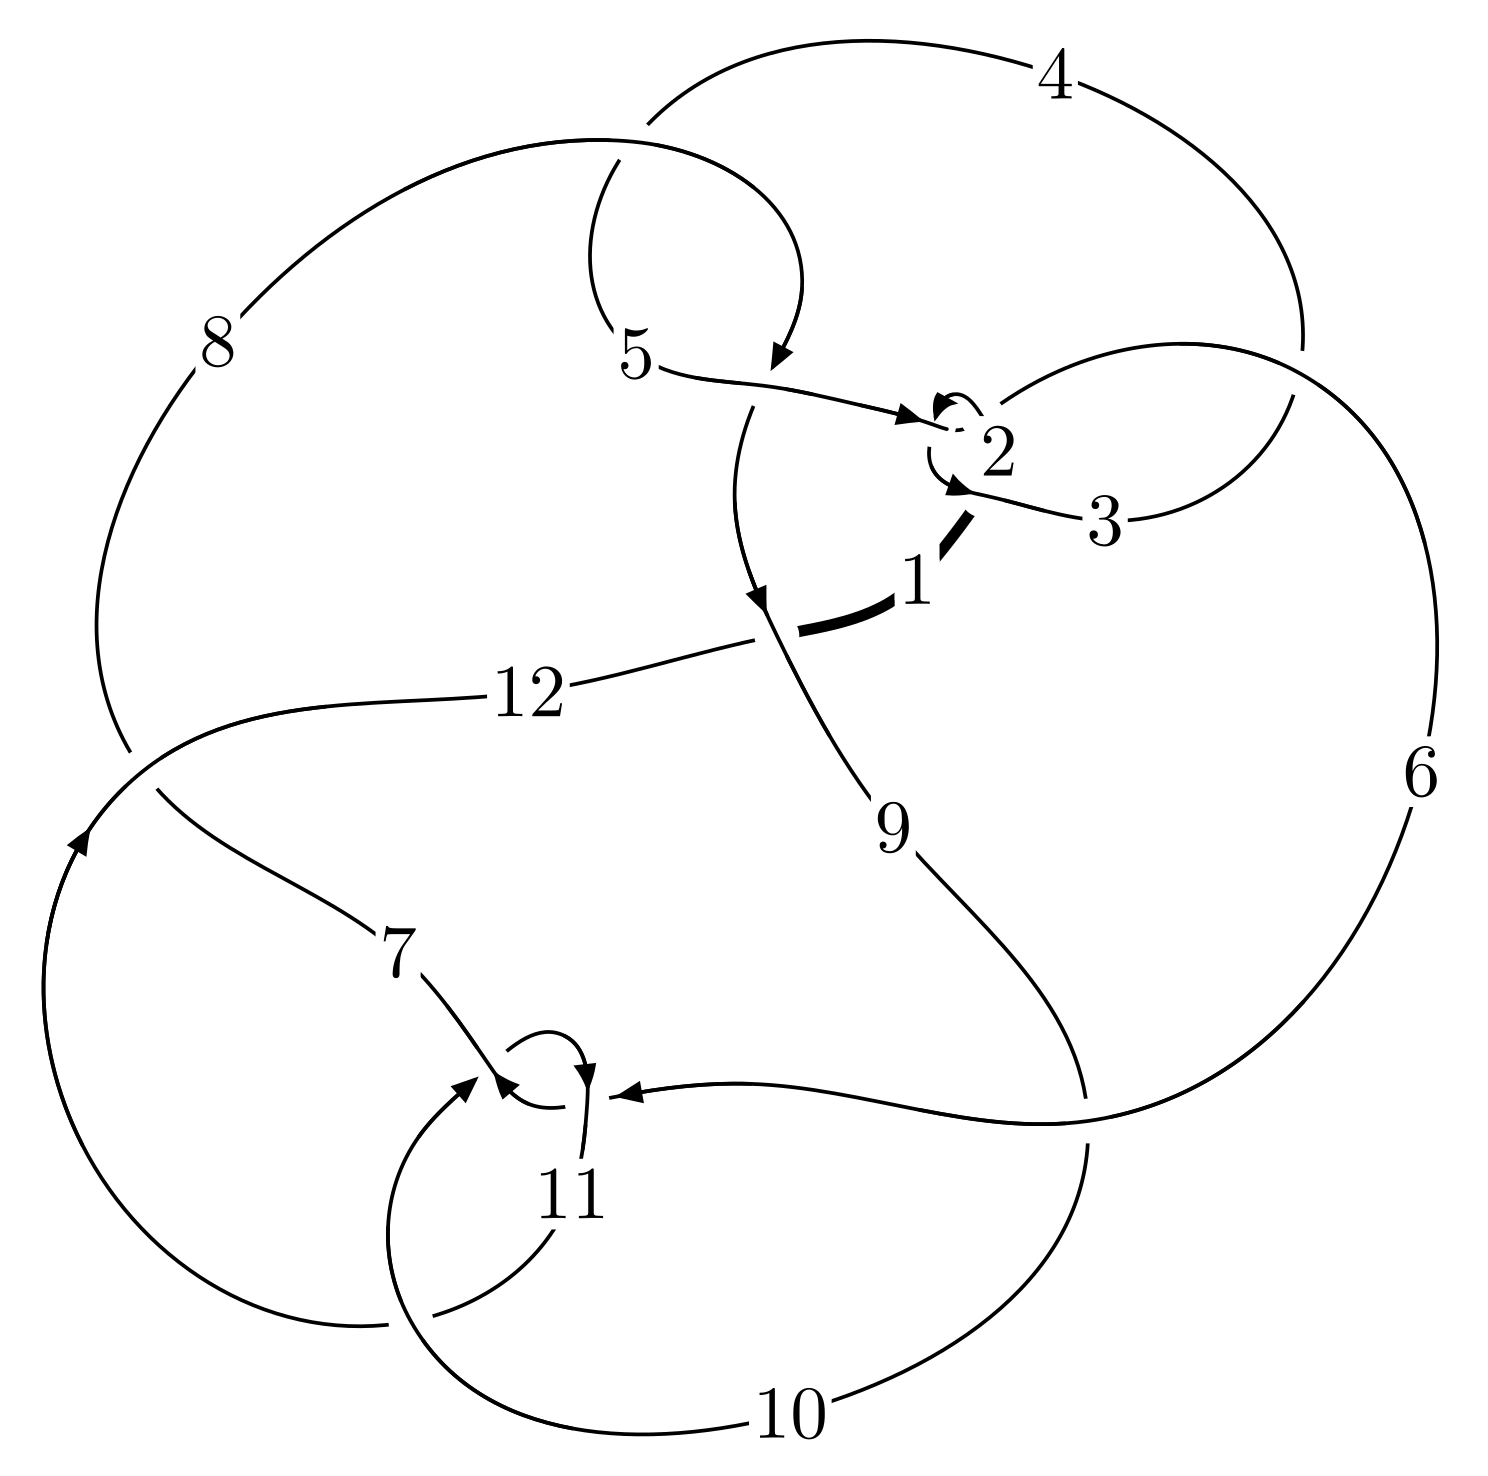
\includegraphics[width=112pt]{../../../GIT/diagram.site/Diagrams/png/2124_12n_0035.png}\\
\ \ \ A knot diagram\footnotemark}&
\allowdisplaybreaks
\textbf{Linearized knot diagam} \\
\cline{2-2}
 &
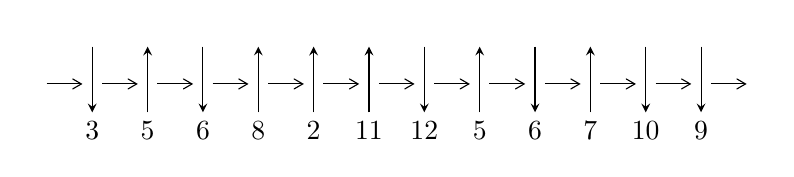
\begin{tikzpicture}[x=20pt, y=17pt]
	% nodes
	\node (C0) at (0, 0) {};
	\node (C1) at (1, 0) {};
	\node (C1U) at (1, +1) {};
	\node (C1D) at (1, -1) {3};

	\node (C2) at (2, 0) {};
	\node (C2U) at (2, +1) {};
	\node (C2D) at (2, -1) {5};

	\node (C3) at (3, 0) {};
	\node (C3U) at (3, +1) {};
	\node (C3D) at (3, -1) {6};

	\node (C4) at (4, 0) {};
	\node (C4U) at (4, +1) {};
	\node (C4D) at (4, -1) {8};

	\node (C5) at (5, 0) {};
	\node (C5U) at (5, +1) {};
	\node (C5D) at (5, -1) {2};

	\node (C6) at (6, 0) {};
	\node (C6U) at (6, +1) {};
	\node (C6D) at (6, -1) {11};

	\node (C7) at (7, 0) {};
	\node (C7U) at (7, +1) {};
	\node (C7D) at (7, -1) {12};

	\node (C8) at (8, 0) {};
	\node (C8U) at (8, +1) {};
	\node (C8D) at (8, -1) {5};

	\node (C9) at (9, 0) {};
	\node (C9U) at (9, +1) {};
	\node (C9D) at (9, -1) {6};

	\node (C10) at (10, 0) {};
	\node (C10U) at (10, +1) {};
	\node (C10D) at (10, -1) {7};

	\node (C11) at (11, 0) {};
	\node (C11U) at (11, +1) {};
	\node (C11D) at (11, -1) {10};

	\node (C12) at (12, 0) {};
	\node (C12U) at (12, +1) {};
	\node (C12D) at (12, -1) {9};
	\node (C13) at (13, 0) {};

	% arrows
	\draw[->,>={angle 60}]
	(C0) edge (C1) (C1) edge (C2) (C2) edge (C3) (C3) edge (C4) (C4) edge (C5) (C5) edge (C6) (C6) edge (C7) (C7) edge (C8) (C8) edge (C9) (C9) edge (C10) (C10) edge (C11) (C11) edge (C12) (C12) edge (C13) ;	\draw[->,>=stealth]
	(C1U) edge (C1D) (C2D) edge (C2U) (C3U) edge (C3D) (C4D) edge (C4U) (C5D) edge (C5U) (C6D) edge (C6U) (C7U) edge (C7D) (C8D) edge (C8U) (C9U) edge (C9D) (C10D) edge (C10U) (C11U) edge (C11D) (C12U) edge (C12D) ;
	\end{tikzpicture} \\
\hhline{~~} \\& 
\textbf{Solving Sequence} \\ \cline{2-2} 
 &
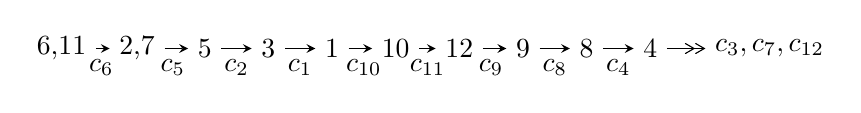
\begin{tikzpicture}[x=23pt, y=7pt]
	% node
	\node (A0) at (-1/8, 0) {6,11};
	\node (A1) at (17/16, 0) {2,7};
	\node (A2) at (17/8, 0) {5};
	\node (A3) at (25/8, 0) {3};
	\node (A4) at (33/8, 0) {1};
	\node (A5) at (41/8, 0) {10};
	\node (A6) at (49/8, 0) {12};
	\node (A7) at (57/8, 0) {9};
	\node (A8) at (65/8, 0) {8};
	\node (A9) at (73/8, 0) {4};
	\node (C1) at (1/2, -1) {$c_{6}$};
	\node (C2) at (13/8, -1) {$c_{5}$};
	\node (C3) at (21/8, -1) {$c_{2}$};
	\node (C4) at (29/8, -1) {$c_{1}$};
	\node (C5) at (37/8, -1) {$c_{10}$};
	\node (C6) at (45/8, -1) {$c_{11}$};
	\node (C7) at (53/8, -1) {$c_{9}$};
	\node (C8) at (61/8, -1) {$c_{8}$};
	\node (C9) at (69/8, -1) {$c_{4}$};
	\node (A10) at (11, 0) {$c_{3},c_{7},c_{12}$};

	% edge
	\draw[->,>=stealth]	
	(A0) edge (A1) (A1) edge (A2) (A2) edge (A3) (A3) edge (A4) (A4) edge (A5) (A5) edge (A6) (A6) edge (A7) (A7) edge (A8) (A8) edge (A9) ;
	\draw[->>,>={angle 60}]	
	(A9) edge (A10);
\end{tikzpicture} \\ 

\end{tabular} \\

\footnotetext{
The image of knot diagram is generated by the software ``\textbf{Draw programme}" developed by Andrew Bartholomew(\url{http://www.layer8.co.uk/maths/draw/index.htm\#Running-draw}), where we modified some parts for our purpose(\url{https://github.com/CATsTAILs/LinksPainter}).
}\phantom \\ \newline 
\centering \textbf{Ideals for irreducible components\footnotemark of $X_{\text{par}}$} 
 
\begin{align*}
I^u_{1}&=\langle 
- u^{42}-2 u^{41}+\cdots+2 b- u,\;-2 u^{42}-4 u^{41}+\cdots+2 a-2,\;u^{44}+3 u^{43}+\cdots+3 u+1\rangle \\
I^u_{2}&=\langle 
-2 u^4 a-4 u^3 a-2 u^4+3 u^2 a-4 u^3-8 a u+3 u^2+19 b-7 a-8 u-7,\\
\phantom{I^u_{2}}&\phantom{= \langle  }u^3 a- u^2 a-2 u^3+a^2+a u+2 u^2- u+2,\;u^5- u^4+2 u^3- u^2+u-1\rangle \\
\\
\end{align*}
\raggedright * 2 irreducible components of $\dim_{\mathbb{C}}=0$, with total 54 representations.\\
\footnotetext{All coefficients of polynomials are rational numbers. But the coefficients are sometimes approximated in decimal forms when there is not enough margin.}
\newpage
\renewcommand{\arraystretch}{1}
\centering \section*{I. $I^u_{1}= \langle - u^{42}-2 u^{41}+\cdots+2 b- u,\;-2 u^{42}-4 u^{41}+\cdots+2 a-2,\;u^{44}+3 u^{43}+\cdots+3 u+1 \rangle$}
\flushleft \textbf{(i) Arc colorings}\\
\begin{tabular}{m{7pt} m{180pt} m{7pt} m{180pt} }
\flushright $a_{6}=$&$\begin{pmatrix}1\\0\end{pmatrix}$ \\
\flushright $a_{11}=$&$\begin{pmatrix}0\\u\end{pmatrix}$ \\
\flushright $a_{2}=$&$\begin{pmatrix}u^{42}+2 u^{41}+\cdots+\frac{1}{2} u+1\\\frac{1}{2} u^{42}+u^{41}+\cdots+u^2+\frac{1}{2} u\end{pmatrix}$ \\
\flushright $a_{7}=$&$\begin{pmatrix}1\\- u^2\end{pmatrix}$ \\
\flushright $a_{5}=$&$\begin{pmatrix}\frac{5}{2} u^{42}+5 u^{41}+\cdots+3 u+1\\\frac{1}{2} u^{42}+u^{41}+\cdots+2 u^2+\frac{3}{2} u\end{pmatrix}$ \\
\flushright $a_{3}=$&$\begin{pmatrix}-3 u^{42}-6 u^{41}+\cdots-\frac{7}{2} u-1\\-\frac{3}{2} u^{42}-2 u^{41}+\cdots-3 u^2-\frac{3}{2} u\end{pmatrix}$ \\
\flushright $a_{1}=$&$\begin{pmatrix}- u^{11}-2 u^9-2 u^7- u^3\\- u^{11}-3 u^9-4 u^7- u^5+u^3+u\end{pmatrix}$ \\
\flushright $a_{10}=$&$\begin{pmatrix}- u\\u^3+u\end{pmatrix}$ \\
\flushright $a_{12}=$&$\begin{pmatrix}- u^3\\u^5+u^3+u\end{pmatrix}$ \\
\flushright $a_{9}=$&$\begin{pmatrix}u^3\\u^3+u\end{pmatrix}$ \\
\flushright $a_{8}=$&$\begin{pmatrix}- u^6- u^4+1\\u^8+2 u^6+2 u^4\end{pmatrix}$ \\
\flushright $a_{4}=$&$\begin{pmatrix}\frac{3}{2} u^{42}+4 u^{41}+\cdots+2 u+1\\\frac{3}{2} u^{42}+2 u^{41}+\cdots+3 u^2+\frac{3}{2} u\end{pmatrix}$\\&\end{tabular}
\flushleft \textbf{(ii) Obstruction class $= -1$}\\~\\
\flushleft \textbf{(iii) Cusp Shapes $= 4 u^{43}+\frac{39}{2} u^{42}+\cdots+25 u+\frac{23}{2}$}\\~\\
\newpage\renewcommand{\arraystretch}{1}
\flushleft \textbf{(iv) u-Polynomials at the component}\newline \\
\begin{tabular}{m{50pt}|m{274pt}}
Crossings & \hspace{64pt}u-Polynomials at each crossing \\
\hline $$\begin{aligned}c_{1}\end{aligned}$$&$\begin{aligned}
&u^{44}+10 u^{43}+\cdots+2 u+1
\end{aligned}$\\
\hline $$\begin{aligned}c_{2},c_{5}\end{aligned}$$&$\begin{aligned}
&u^{44}+6 u^{43}+\cdots+6 u+1
\end{aligned}$\\
\hline $$\begin{aligned}c_{3}\end{aligned}$$&$\begin{aligned}
&u^{44}-6 u^{43}+\cdots+717363 u+73746
\end{aligned}$\\
\hline $$\begin{aligned}c_{4},c_{8}\end{aligned}$$&$\begin{aligned}
&u^{44}- u^{43}+\cdots+1024 u+1024
\end{aligned}$\\
\hline $$\begin{aligned}c_{6},c_{10}\end{aligned}$$&$\begin{aligned}
&u^{44}-3 u^{43}+\cdots-3 u+1
\end{aligned}$\\
\hline $$\begin{aligned}c_{7},c_{9}\end{aligned}$$&$\begin{aligned}
&u^{44}+3 u^{43}+\cdots+211 u+34
\end{aligned}$\\
\hline $$\begin{aligned}c_{11}\end{aligned}$$&$\begin{aligned}
&u^{44}+23 u^{43}+\cdots+3 u+1
\end{aligned}$\\
\hline $$\begin{aligned}c_{12}\end{aligned}$$&$\begin{aligned}
&u^{44}- u^{43}+\cdots+3 u+1
\end{aligned}$\\
\hline
\end{tabular}\\~\\
\newpage\renewcommand{\arraystretch}{1}
\flushleft \textbf{(v) Riley Polynomials at the component}\newline \\
\begin{tabular}{m{50pt}|m{274pt}}
Crossings & \hspace{64pt}Riley Polynomials at each crossing \\
\hline $$\begin{aligned}c_{1}\end{aligned}$$&$\begin{aligned}
&y^{44}+54 y^{43}+\cdots+102 y+1
\end{aligned}$\\
\hline $$\begin{aligned}c_{2},c_{5}\end{aligned}$$&$\begin{aligned}
&y^{44}+10 y^{43}+\cdots+2 y+1
\end{aligned}$\\
\hline $$\begin{aligned}c_{3}\end{aligned}$$&$\begin{aligned}
&y^{44}+98 y^{43}+\cdots+113290466283 y+5438472516
\end{aligned}$\\
\hline $$\begin{aligned}c_{4},c_{8}\end{aligned}$$&$\begin{aligned}
&y^{44}-55 y^{43}+\cdots-1048576 y+1048576
\end{aligned}$\\
\hline $$\begin{aligned}c_{6},c_{10}\end{aligned}$$&$\begin{aligned}
&y^{44}+23 y^{43}+\cdots+3 y+1
\end{aligned}$\\
\hline $$\begin{aligned}c_{7},c_{9}\end{aligned}$$&$\begin{aligned}
&y^{44}-25 y^{43}+\cdots+17903 y+1156
\end{aligned}$\\
\hline $$\begin{aligned}c_{11}\end{aligned}$$&$\begin{aligned}
&y^{44}- y^{43}+\cdots+11 y+1
\end{aligned}$\\
\hline $$\begin{aligned}c_{12}\end{aligned}$$&$\begin{aligned}
&y^{44}+75 y^{43}+\cdots+3 y+1
\end{aligned}$\\
\hline
\end{tabular}\\~\\
\newpage\flushleft \textbf{(vi) Complex Volumes and Cusp Shapes}
$$\begin{array}{c|c|c}  
\text{Solutions to }I^u_{1}& \I (\text{vol} + \sqrt{-1}CS) & \text{Cusp shape}\\
 \hline 
\begin{aligned}
u &= \phantom{-}0.691393 + 0.770310 I \\
a &= -0.066986 + 0.372800 I \\
b &= \phantom{-}0.965189 - 0.946149 I\end{aligned}
 & \phantom{-}11.85400 - 0.89687 I & \phantom{-}3.89150 - 0.58111 I \\ \hline\begin{aligned}
u &= \phantom{-}0.691393 - 0.770310 I \\
a &= -0.066986 - 0.372800 I \\
b &= \phantom{-}0.965189 + 0.946149 I\end{aligned}
 & \phantom{-}11.85400 + 0.89687 I & \phantom{-}3.89150 + 0.58111 I \\ \hline\begin{aligned}
u &= \phantom{-}0.681315 + 0.809304 I \\
a &= -1.36604 + 1.02725 I \\
b &= \phantom{-}0.945813 + 0.981170 I\end{aligned}
 & \phantom{-}11.73940 + 6.10553 I & \phantom{-}3.57078 - 5.20880 I \\ \hline\begin{aligned}
u &= \phantom{-}0.681315 - 0.809304 I \\
a &= -1.36604 - 1.02725 I \\
b &= \phantom{-}0.945813 - 0.981170 I\end{aligned}
 & \phantom{-}11.73940 - 6.10553 I & \phantom{-}3.57078 + 5.20880 I \\ \hline\begin{aligned}
u &= -0.417026 + 0.814240 I \\
a &= -0.966326 - 0.411751 I \\
b &= \phantom{-}0.276291 - 0.156022 I\end{aligned}
 & -0.06080 - 1.78150 I & \phantom{-}0.19283 + 3.69450 I \\ \hline\begin{aligned}
u &= -0.417026 - 0.814240 I \\
a &= -0.966326 + 0.411751 I \\
b &= \phantom{-}0.276291 + 0.156022 I\end{aligned}
 & -0.06080 + 1.78150 I & \phantom{-}0.19283 - 3.69450 I \\ \hline\begin{aligned}
u &= -0.849289 + 0.246416 I \\
a &= -0.864419 + 0.930692 I \\
b &= \phantom{-}0.878595 + 1.030530 I\end{aligned}
 & \phantom{-}8.55506 + 8.32906 I & \phantom{-}2.52276 - 4.33779 I \\ \hline\begin{aligned}
u &= -0.849289 - 0.246416 I \\
a &= -0.864419 - 0.930692 I \\
b &= \phantom{-}0.878595 - 1.030530 I\end{aligned}
 & \phantom{-}8.55506 - 8.32906 I & \phantom{-}2.52276 + 4.33779 I \\ \hline\begin{aligned}
u &= -0.836265 + 0.281412 I \\
a &= -0.206151 - 0.049476 I \\
b &= \phantom{-}0.974475 - 0.853175 I\end{aligned}
 & \phantom{-}9.13585 + 1.52647 I & \phantom{-}3.42363 + 0.21688 I \\ \hline\begin{aligned}
u &= -0.836265 - 0.281412 I \\
a &= -0.206151 + 0.049476 I \\
b &= \phantom{-}0.974475 + 0.853175 I\end{aligned}
 & \phantom{-}9.13585 - 1.52647 I & \phantom{-}3.42363 - 0.21688 I\\
 \hline 
 \end{array}$$\newpage$$\begin{array}{c|c|c}  
\text{Solutions to }I^u_{1}& \I (\text{vol} + \sqrt{-1}CS) & \text{Cusp shape}\\
 \hline 
\begin{aligned}
u &= \phantom{-}0.433525 + 1.047130 I \\
a &= -0.326846 + 0.375439 I \\
b &= -0.695543 + 0.930432 I\end{aligned}
 & -1.29668 + 0.57558 I & -2.65523 - 2.16561 I \\ \hline\begin{aligned}
u &= \phantom{-}0.433525 - 1.047130 I \\
a &= -0.326846 - 0.375439 I \\
b &= -0.695543 - 0.930432 I\end{aligned}
 & -1.29668 - 0.57558 I & -2.65523 + 2.16561 I \\ \hline\begin{aligned}
u &= -0.094054 + 0.853687 I \\
a &= -1.11225 + 1.86145 I \\
b &= -0.198619 + 0.750506 I\end{aligned}
 & -1.66817 - 1.59205 I & -6.58514 + 4.39514 I \\ \hline\begin{aligned}
u &= -0.094054 - 0.853687 I \\
a &= -1.11225 - 1.86145 I \\
b &= -0.198619 - 0.750506 I\end{aligned}
 & -1.66817 + 1.59205 I & -6.58514 - 4.39514 I \\ \hline\begin{aligned}
u &= -0.487271 + 1.047260 I \\
a &= -0.779531 + 0.841946 I \\
b &= -0.766362 - 0.217429 I\end{aligned}
 & -0.23513 - 3.16229 I & \phantom{-}1.52764 + 3.47706 I \\ \hline\begin{aligned}
u &= -0.487271 - 1.047260 I \\
a &= -0.779531 - 0.841946 I \\
b &= -0.766362 + 0.217429 I\end{aligned}
 & -0.23513 + 3.16229 I & \phantom{-}1.52764 - 3.47706 I \\ \hline\begin{aligned}
u &= -0.388702 + 1.120050 I \\
a &= -1.03941 - 2.62383 I \\
b &= -0.288878 - 1.073200 I\end{aligned}
 & -4.05811 - 0.18233 I & -4.90447 + 0. I\phantom{ +0.000000I} \\ \hline\begin{aligned}
u &= -0.388702 - 1.120050 I \\
a &= -1.03941 + 2.62383 I \\
b &= -0.288878 + 1.073200 I\end{aligned}
 & -4.05811 + 0.18233 I & -4.90447 + 0. I\phantom{ +0.000000I} \\ \hline\begin{aligned}
u &= \phantom{-}0.497679 + 1.078530 I \\
a &= \phantom{-}1.02995 - 1.29852 I \\
b &= -0.800804 - 0.775068 I\end{aligned}
 & -0.74030 + 6.20071 I & \phantom{-0.000000 } 0. - 7.00102 I \\ \hline\begin{aligned}
u &= \phantom{-}0.497679 - 1.078530 I \\
a &= \phantom{-}1.02995 + 1.29852 I \\
b &= -0.800804 + 0.775068 I\end{aligned}
 & -0.74030 - 6.20071 I & \phantom{-0.000000 -}0. + 7.00102 I\\
 \hline 
 \end{array}$$\newpage$$\begin{array}{c|c|c}  
\text{Solutions to }I^u_{1}& \I (\text{vol} + \sqrt{-1}CS) & \text{Cusp shape}\\
 \hline 
\begin{aligned}
u &= \phantom{-}0.769712 + 0.052444 I \\
a &= -0.818253 - 0.833331 I \\
b &= \phantom{-}0.257390 - 0.588680 I\end{aligned}
 & -2.66109 - 0.97035 I & -2.65239 - 1.69439 I \\ \hline\begin{aligned}
u &= \phantom{-}0.769712 - 0.052444 I \\
a &= -0.818253 + 0.833331 I \\
b &= \phantom{-}0.257390 + 0.588680 I\end{aligned}
 & -2.66109 + 0.97035 I & -2.65239 + 1.69439 I \\ \hline\begin{aligned}
u &= -0.496317 + 1.126200 I \\
a &= \phantom{-}1.35629 + 2.84442 I \\
b &= -0.396506 + 1.136040 I\end{aligned}
 & -3.29384 - 7.52516 I & \phantom{-0.000000 -}0. + 7.24279 I \\ \hline\begin{aligned}
u &= -0.496317 - 1.126200 I \\
a &= \phantom{-}1.35629 - 2.84442 I \\
b &= -0.396506 - 1.136040 I\end{aligned}
 & -3.29384 + 7.52516 I & \phantom{-0.000000 } 0. - 7.24279 I \\ \hline\begin{aligned}
u &= -0.254712 + 1.221060 I \\
a &= \phantom{-}0.54185 - 1.65734 I \\
b &= \phantom{-}0.918787 - 0.852340 I\end{aligned}
 & \phantom{-}4.30712 - 1.86418 I & \phantom{-0.000000 } 0 \\ \hline\begin{aligned}
u &= -0.254712 - 1.221060 I \\
a &= \phantom{-}0.54185 + 1.65734 I \\
b &= \phantom{-}0.918787 + 0.852340 I\end{aligned}
 & \phantom{-}4.30712 + 1.86418 I & \phantom{-0.000000 } 0 \\ \hline\begin{aligned}
u &= -0.287527 + 1.233810 I \\
a &= \phantom{-}0.72859 + 1.68616 I \\
b &= \phantom{-}0.853738 + 1.000090 I\end{aligned}
 & \phantom{-}3.83508 + 4.68909 I & \phantom{-0.000000 } 0 \\ \hline\begin{aligned}
u &= -0.287527 - 1.233810 I \\
a &= \phantom{-}0.72859 - 1.68616 I \\
b &= \phantom{-}0.853738 - 1.000090 I\end{aligned}
 & \phantom{-}3.83508 - 4.68909 I & \phantom{-0.000000 } 0 \\ \hline\begin{aligned}
u &= \phantom{-}0.433746 + 1.198270 I \\
a &= -0.009131 - 1.365560 I \\
b &= \phantom{-}0.240844 - 0.671835 I\end{aligned}
 & -6.28026 + 3.26453 I & \phantom{-0.000000 } 0 \\ \hline\begin{aligned}
u &= \phantom{-}0.433746 - 1.198270 I \\
a &= -0.009131 + 1.365560 I \\
b &= \phantom{-}0.240844 + 0.671835 I\end{aligned}
 & -6.28026 - 3.26453 I & \phantom{-0.000000 } 0\\
 \hline 
 \end{array}$$\newpage$$\begin{array}{c|c|c}  
\text{Solutions to }I^u_{1}& \I (\text{vol} + \sqrt{-1}CS) & \text{Cusp shape}\\
 \hline 
\begin{aligned}
u &= \phantom{-}0.474335 + 1.198320 I \\
a &= -0.95599 + 1.60970 I \\
b &= \phantom{-}0.327962 + 0.610342 I\end{aligned}
 & -5.99302 + 5.51262 I & \phantom{-0.000000 } 0 \\ \hline\begin{aligned}
u &= \phantom{-}0.474335 - 1.198320 I \\
a &= -0.95599 - 1.60970 I \\
b &= \phantom{-}0.327962 - 0.610342 I\end{aligned}
 & -5.99302 - 5.51262 I & \phantom{-0.000000 } 0 \\ \hline\begin{aligned}
u &= -0.572998 + 1.165320 I \\
a &= \phantom{-}1.218420 - 0.246333 I \\
b &= \phantom{-}0.988002 + 0.822945 I\end{aligned}
 & \phantom{-}6.50379 - 6.73509 I & \phantom{-0.000000 } 0 \\ \hline\begin{aligned}
u &= -0.572998 - 1.165320 I \\
a &= \phantom{-}1.218420 + 0.246333 I \\
b &= \phantom{-}0.988002 - 0.822945 I\end{aligned}
 & \phantom{-}6.50379 + 6.73509 I & \phantom{-0.000000 } 0 \\ \hline\begin{aligned}
u &= -0.563792 + 1.182090 I \\
a &= -1.12741 - 2.43594 I \\
b &= \phantom{-}0.865756 - 1.050490 I\end{aligned}
 & \phantom{-}5.7613 - 13.5297 I & \phantom{-0.000000 } 0 \\ \hline\begin{aligned}
u &= -0.563792 - 1.182090 I \\
a &= -1.12741 + 2.43594 I \\
b &= \phantom{-}0.865756 + 1.050490 I\end{aligned}
 & \phantom{-}5.7613 + 13.5297 I & \phantom{-0.000000 } 0 \\ \hline\begin{aligned}
u &= -0.519184 + 0.444465 I \\
a &= \phantom{-}0.243564 - 0.426397 I \\
b &= -0.671501 + 0.420740 I\end{aligned}
 & \phantom{-}1.51555 - 0.97971 I & \phantom{-}5.31353 + 2.39080 I \\ \hline\begin{aligned}
u &= -0.519184 - 0.444465 I \\
a &= \phantom{-}0.243564 + 0.426397 I \\
b &= -0.671501 - 0.420740 I\end{aligned}
 & \phantom{-}1.51555 + 0.97971 I & \phantom{-}5.31353 - 2.39080 I \\ \hline\begin{aligned}
u &= \phantom{-}0.363275 + 0.565886 I \\
a &= \phantom{-}2.00200 - 1.16729 I \\
b &= -0.553077 - 0.974993 I\end{aligned}
 & \phantom{-}0.28460 + 2.90693 I & \phantom{-}3.00949 - 1.23686 I \\ \hline\begin{aligned}
u &= \phantom{-}0.363275 - 0.565886 I \\
a &= \phantom{-}2.00200 + 1.16729 I \\
b &= -0.553077 + 0.974993 I\end{aligned}
 & \phantom{-}0.28460 - 2.90693 I & \phantom{-}3.00949 + 1.23686 I\\
 \hline 
 \end{array}$$\newpage$$\begin{array}{c|c|c}  
\text{Solutions to }I^u_{1}& \I (\text{vol} + \sqrt{-1}CS) & \text{Cusp shape}\\
 \hline 
\begin{aligned}
u &= \phantom{-}0.539085 + 0.365328 I \\
a &= \phantom{-}0.768774 - 0.591177 I \\
b &= -0.715038 + 0.680296 I\end{aligned}
 & \phantom{-}1.31536 - 1.96169 I & \phantom{-}3.58238 + 3.39063 I \\ \hline\begin{aligned}
u &= \phantom{-}0.539085 - 0.365328 I \\
a &= \phantom{-}0.768774 + 0.591177 I \\
b &= -0.715038 - 0.680296 I\end{aligned}
 & \phantom{-}1.31536 + 1.96169 I & \phantom{-}3.58238 - 3.39063 I \\ \hline\begin{aligned}
u &= -0.616927 + 0.185561 I \\
a &= \phantom{-}0.74931 - 1.75287 I \\
b &= -0.406514 - 1.058610 I\end{aligned}
 & -0.68635 + 3.17011 I & \phantom{-}1.49231 - 4.26381 I \\ \hline\begin{aligned}
u &= -0.616927 - 0.185561 I \\
a &= \phantom{-}0.74931 + 1.75287 I \\
b &= -0.406514 + 1.058610 I\end{aligned}
 & -0.68635 - 3.17011 I & \phantom{-}1.49231 + 4.26381 I\\
 \hline 
 \end{array}$$\newpage\newpage\renewcommand{\arraystretch}{1}
\centering \section*{II. $I^u_{2}= \langle -2 u^4 a-2 u^4+\cdots-7 a-7,\;u^3 a- u^2 a-2 u^3+a^2+a u+2 u^2- u+2,\;u^5- u^4+2 u^3- u^2+u-1 \rangle$}
\flushleft \textbf{(i) Arc colorings}\\
\begin{tabular}{m{7pt} m{180pt} m{7pt} m{180pt} }
\flushright $a_{6}=$&$\begin{pmatrix}1\\0\end{pmatrix}$ \\
\flushright $a_{11}=$&$\begin{pmatrix}0\\u\end{pmatrix}$ \\
\flushright $a_{2}=$&$\begin{pmatrix}a\\0.105263 a u^{4}+0.105263 u^{4}+\cdots+0.368421 a+0.368421\end{pmatrix}$ \\
\flushright $a_{7}=$&$\begin{pmatrix}1\\- u^2\end{pmatrix}$ \\
\flushright $a_{5}=$&$\begin{pmatrix}-0.105263 a u^{4}-0.105263 u^{4}+\cdots+0.631579 a-0.368421\\0.105263 a u^{4}+0.105263 u^{4}+\cdots+0.368421 a-0.631579\end{pmatrix}$ \\
\flushright $a_{3}=$&$\begin{pmatrix}u^3- u^2+a+u-1\\0.105263 a u^{4}+0.105263 u^{4}+\cdots+0.368421 a-0.631579\end{pmatrix}$ \\
\flushright $a_{1}=$&$\begin{pmatrix}-1\\0\end{pmatrix}$ \\
\flushright $a_{10}=$&$\begin{pmatrix}- u\\u^3+u\end{pmatrix}$ \\
\flushright $a_{12}=$&$\begin{pmatrix}- u^3\\u^4- u^3+u^2+1\end{pmatrix}$ \\
\flushright $a_{9}=$&$\begin{pmatrix}u^3\\u^3+u\end{pmatrix}$ \\
\flushright $a_{8}=$&$\begin{pmatrix}u^3\\u^3+u\end{pmatrix}$ \\
\flushright $a_{4}=$&$\begin{pmatrix}-0.105263 a u^{4}-0.105263 u^{4}+\cdots+0.631579 a-0.368421\\0.105263 a u^{4}+0.105263 u^{4}+\cdots+0.368421 a-0.631579\end{pmatrix}$\\&\end{tabular}
\flushleft \textbf{(ii) Obstruction class $= 1$}\\~\\
\flushleft \textbf{(iii) Cusp Shapes $= - u^4 a- u^3 a+u^2 a+2 u^3-3 a u-2 u^2- a+u-2$}\\~\\
\newpage\renewcommand{\arraystretch}{1}
\flushleft \textbf{(iv) u-Polynomials at the component}\newline \\
\begin{tabular}{m{50pt}|m{274pt}}
Crossings & \hspace{64pt}u-Polynomials at each crossing \\
\hline $$\begin{aligned}c_{1},c_{3},c_{5}\end{aligned}$$&$\begin{aligned}
&(u^2- u+1)^5
\end{aligned}$\\
\hline $$\begin{aligned}c_{2}\end{aligned}$$&$\begin{aligned}
&(u^2+u+1)^5
\end{aligned}$\\
\hline $$\begin{aligned}c_{4},c_{8}\end{aligned}$$&$\begin{aligned}
&u^{10}
\end{aligned}$\\
\hline $$\begin{aligned}c_{6}\end{aligned}$$&$\begin{aligned}
&(u^5- u^4+2 u^3- u^2+u-1)^2
\end{aligned}$\\
\hline $$\begin{aligned}c_{7}\end{aligned}$$&$\begin{aligned}
&(u^5+u^4-2 u^3- u^2+u-1)^2
\end{aligned}$\\
\hline $$\begin{aligned}c_{9},c_{12}\end{aligned}$$&$\begin{aligned}
&(u^5- u^4-2 u^3+u^2+u+1)^2
\end{aligned}$\\
\hline $$\begin{aligned}c_{10}\end{aligned}$$&$\begin{aligned}
&(u^5+u^4+2 u^3+u^2+u+1)^2
\end{aligned}$\\
\hline $$\begin{aligned}c_{11}\end{aligned}$$&$\begin{aligned}
&(u^5+3 u^4+4 u^3+u^2- u-1)^2
\end{aligned}$\\
\hline
\end{tabular}\\~\\
\newpage\renewcommand{\arraystretch}{1}
\flushleft \textbf{(v) Riley Polynomials at the component}\newline \\
\begin{tabular}{m{50pt}|m{274pt}}
Crossings & \hspace{64pt}Riley Polynomials at each crossing \\
\hline $$\begin{aligned}c_{1},c_{2},c_{3}\\c_{5}\end{aligned}$$&$\begin{aligned}
&(y^2+y+1)^5
\end{aligned}$\\
\hline $$\begin{aligned}c_{4},c_{8}\end{aligned}$$&$\begin{aligned}
&y^{10}
\end{aligned}$\\
\hline $$\begin{aligned}c_{6},c_{10}\end{aligned}$$&$\begin{aligned}
&(y^5+3 y^4+4 y^3+y^2- y-1)^2
\end{aligned}$\\
\hline $$\begin{aligned}c_{7},c_{9},c_{12}\end{aligned}$$&$\begin{aligned}
&(y^5-5 y^4+8 y^3-3 y^2- y-1)^2
\end{aligned}$\\
\hline $$\begin{aligned}c_{11}\end{aligned}$$&$\begin{aligned}
&(y^5- y^4+8 y^3-3 y^2+3 y-1)^2
\end{aligned}$\\
\hline
\end{tabular}\\~\\
\newpage\flushleft \textbf{(vi) Complex Volumes and Cusp Shapes}
$$\begin{array}{c|c|c}  
\text{Solutions to }I^u_{2}& \I (\text{vol} + \sqrt{-1}CS) & \text{Cusp shape}\\
 \hline 
\begin{aligned}
u &= -0.339110 + 0.822375 I \\
a &= \phantom{-}0.523653 + 0.423720 I \\
b &= \phantom{-}0.500000 + 0.866025 I\end{aligned}
 & -0.329100 + 0.499304 I & \phantom{-}0.886311 - 0.883423 I \\ \hline\begin{aligned}
u &= -0.339110 + 0.822375 I \\
a &= -1.39487 - 1.53138 I \\
b &= \phantom{-}0.500000 - 0.866025 I\end{aligned}
 & -0.32910 - 3.56046 I & -3.42267 + 7.93863 I \\ \hline\begin{aligned}
u &= -0.339110 - 0.822375 I \\
a &= \phantom{-}0.523653 - 0.423720 I \\
b &= \phantom{-}0.500000 - 0.866025 I\end{aligned}
 & -0.329100 - 0.499304 I & \phantom{-}0.886311 + 0.883423 I \\ \hline\begin{aligned}
u &= -0.339110 - 0.822375 I \\
a &= -1.39487 + 1.53138 I \\
b &= \phantom{-}0.500000 + 0.866025 I\end{aligned}
 & -0.32910 + 3.56046 I & -3.42267 - 7.93863 I \\ \hline\begin{aligned}
u &= \phantom{-}0.766826\phantom{ +0.000000I} \\
a &= -0.314857 + 1.186700 I \\
b &= \phantom{-}0.500000 + 0.866025 I\end{aligned}
 & -2.40108 + 2.02988 I & -0.40252 - 4.16430 I \\ \hline\begin{aligned}
u &= \phantom{-}0.766826\phantom{ +0.000000I} \\
a &= -0.314857 - 1.186700 I \\
b &= \phantom{-}0.500000 - 0.866025 I\end{aligned}
 & -2.40108 - 2.02988 I & -0.40252 + 4.16430 I \\ \hline\begin{aligned}
u &= \phantom{-}0.455697 + 1.200150 I \\
a &= \phantom{-}0.85051 - 1.45588 I \\
b &= \phantom{-}0.500000 - 0.866025 I\end{aligned}
 & -5.87256 + 2.37095 I & -2.86519 + 1.02882 I \\ \hline\begin{aligned}
u &= \phantom{-}0.455697 + 1.200150 I \\
a &= -0.66443 + 2.33052 I \\
b &= \phantom{-}0.500000 + 0.866025 I\end{aligned}
 & -5.87256 + 6.43072 I & -4.19593 - 8.50148 I \\ \hline\begin{aligned}
u &= \phantom{-}0.455697 - 1.200150 I \\
a &= \phantom{-}0.85051 + 1.45588 I \\
b &= \phantom{-}0.500000 + 0.866025 I\end{aligned}
 & -5.87256 - 2.37095 I & -2.86519 - 1.02882 I \\ \hline\begin{aligned}
u &= \phantom{-}0.455697 - 1.200150 I \\
a &= -0.66443 - 2.33052 I \\
b &= \phantom{-}0.500000 - 0.866025 I\end{aligned}
 & -5.87256 - 6.43072 I & -4.19593 + 8.50148 I\\
 \hline 
 \end{array}$$\newpage
\newpage\renewcommand{\arraystretch}{1}
\centering \section*{ III. u-Polynomials}
\begin{tabular}{m{50pt}|m{274pt}}
Crossings & \hspace{64pt}u-Polynomials at each crossing \\
\hline $$\begin{aligned}c_{1}\end{aligned}$$&$\begin{aligned}
&((u^2- u+1)^5)(u^{44}+10 u^{43}+\cdots+2 u+1)
\end{aligned}$\\
\hline $$\begin{aligned}c_{2}\end{aligned}$$&$\begin{aligned}
&((u^2+u+1)^5)(u^{44}+6 u^{43}+\cdots+6 u+1)
\end{aligned}$\\
\hline $$\begin{aligned}c_{3}\end{aligned}$$&$\begin{aligned}
&((u^2- u+1)^5)(u^{44}-6 u^{43}+\cdots+717363 u+73746)
\end{aligned}$\\
\hline $$\begin{aligned}c_{4},c_{8}\end{aligned}$$&$\begin{aligned}
&u^{10}(u^{44}- u^{43}+\cdots+1024 u+1024)
\end{aligned}$\\
\hline $$\begin{aligned}c_{5}\end{aligned}$$&$\begin{aligned}
&((u^2- u+1)^5)(u^{44}+6 u^{43}+\cdots+6 u+1)
\end{aligned}$\\
\hline $$\begin{aligned}c_{6}\end{aligned}$$&$\begin{aligned}
&((u^5- u^4+2 u^3- u^2+u-1)^2)(u^{44}-3 u^{43}+\cdots-3 u+1)
\end{aligned}$\\
\hline $$\begin{aligned}c_{7}\end{aligned}$$&$\begin{aligned}
&((u^5+u^4-2 u^3- u^2+u-1)^2)(u^{44}+3 u^{43}+\cdots+211 u+34)
\end{aligned}$\\
\hline $$\begin{aligned}c_{9}\end{aligned}$$&$\begin{aligned}
&((u^5- u^4-2 u^3+u^2+u+1)^2)(u^{44}+3 u^{43}+\cdots+211 u+34)
\end{aligned}$\\
\hline $$\begin{aligned}c_{10}\end{aligned}$$&$\begin{aligned}
&((u^5+u^4+2 u^3+u^2+u+1)^2)(u^{44}-3 u^{43}+\cdots-3 u+1)
\end{aligned}$\\
\hline $$\begin{aligned}c_{11}\end{aligned}$$&$\begin{aligned}
&((u^5+3 u^4+4 u^3+u^2- u-1)^2)(u^{44}+23 u^{43}+\cdots+3 u+1)
\end{aligned}$\\
\hline $$\begin{aligned}c_{12}\end{aligned}$$&$\begin{aligned}
&((u^5- u^4-2 u^3+u^2+u+1)^2)(u^{44}- u^{43}+\cdots+3 u+1)
\end{aligned}$\\
\hline
\end{tabular}\newpage\renewcommand{\arraystretch}{1}
\centering \section*{ IV. Riley Polynomials}
\begin{tabular}{m{50pt}|m{274pt}}
Crossings & \hspace{64pt}Riley Polynomials at each crossing \\
\hline $$\begin{aligned}c_{1}\end{aligned}$$&$\begin{aligned}
&((y^2+y+1)^5)(y^{44}+54 y^{43}+\cdots+102 y+1)
\end{aligned}$\\
\hline $$\begin{aligned}c_{2},c_{5}\end{aligned}$$&$\begin{aligned}
&((y^2+y+1)^5)(y^{44}+10 y^{43}+\cdots+2 y+1)
\end{aligned}$\\
\hline $$\begin{aligned}c_{3}\end{aligned}$$&$\begin{aligned}
&((y^2+y+1)^5)(y^{44}+98 y^{43}+\cdots+1.13290\times10^{11} y+5.43847\times10^{9})
\end{aligned}$\\
\hline $$\begin{aligned}c_{4},c_{8}\end{aligned}$$&$\begin{aligned}
&y^{10}(y^{44}-55 y^{43}+\cdots-1048576 y+1048576)
\end{aligned}$\\
\hline $$\begin{aligned}c_{6},c_{10}\end{aligned}$$&$\begin{aligned}
&((y^5+3 y^4+4 y^3+y^2- y-1)^2)(y^{44}+23 y^{43}+\cdots+3 y+1)
\end{aligned}$\\
\hline $$\begin{aligned}c_{7},c_{9}\end{aligned}$$&$\begin{aligned}
&((y^5-5 y^4+8 y^3-3 y^2- y-1)^2)(y^{44}-25 y^{43}+\cdots+17903 y+1156)
\end{aligned}$\\
\hline $$\begin{aligned}c_{11}\end{aligned}$$&$\begin{aligned}
&((y^5- y^4+8 y^3-3 y^2+3 y-1)^2)(y^{44}- y^{43}+\cdots+11 y+1)
\end{aligned}$\\
\hline $$\begin{aligned}c_{12}\end{aligned}$$&$\begin{aligned}
&((y^5-5 y^4+8 y^3-3 y^2- y-1)^2)(y^{44}+75 y^{43}+\cdots+3 y+1)
\end{aligned}$\\
\hline
\end{tabular}
\vskip 2pc
\end{document}